\begin{figure*}[tb]
 \begin{subfigure}{\columnwidth}
 \centering
 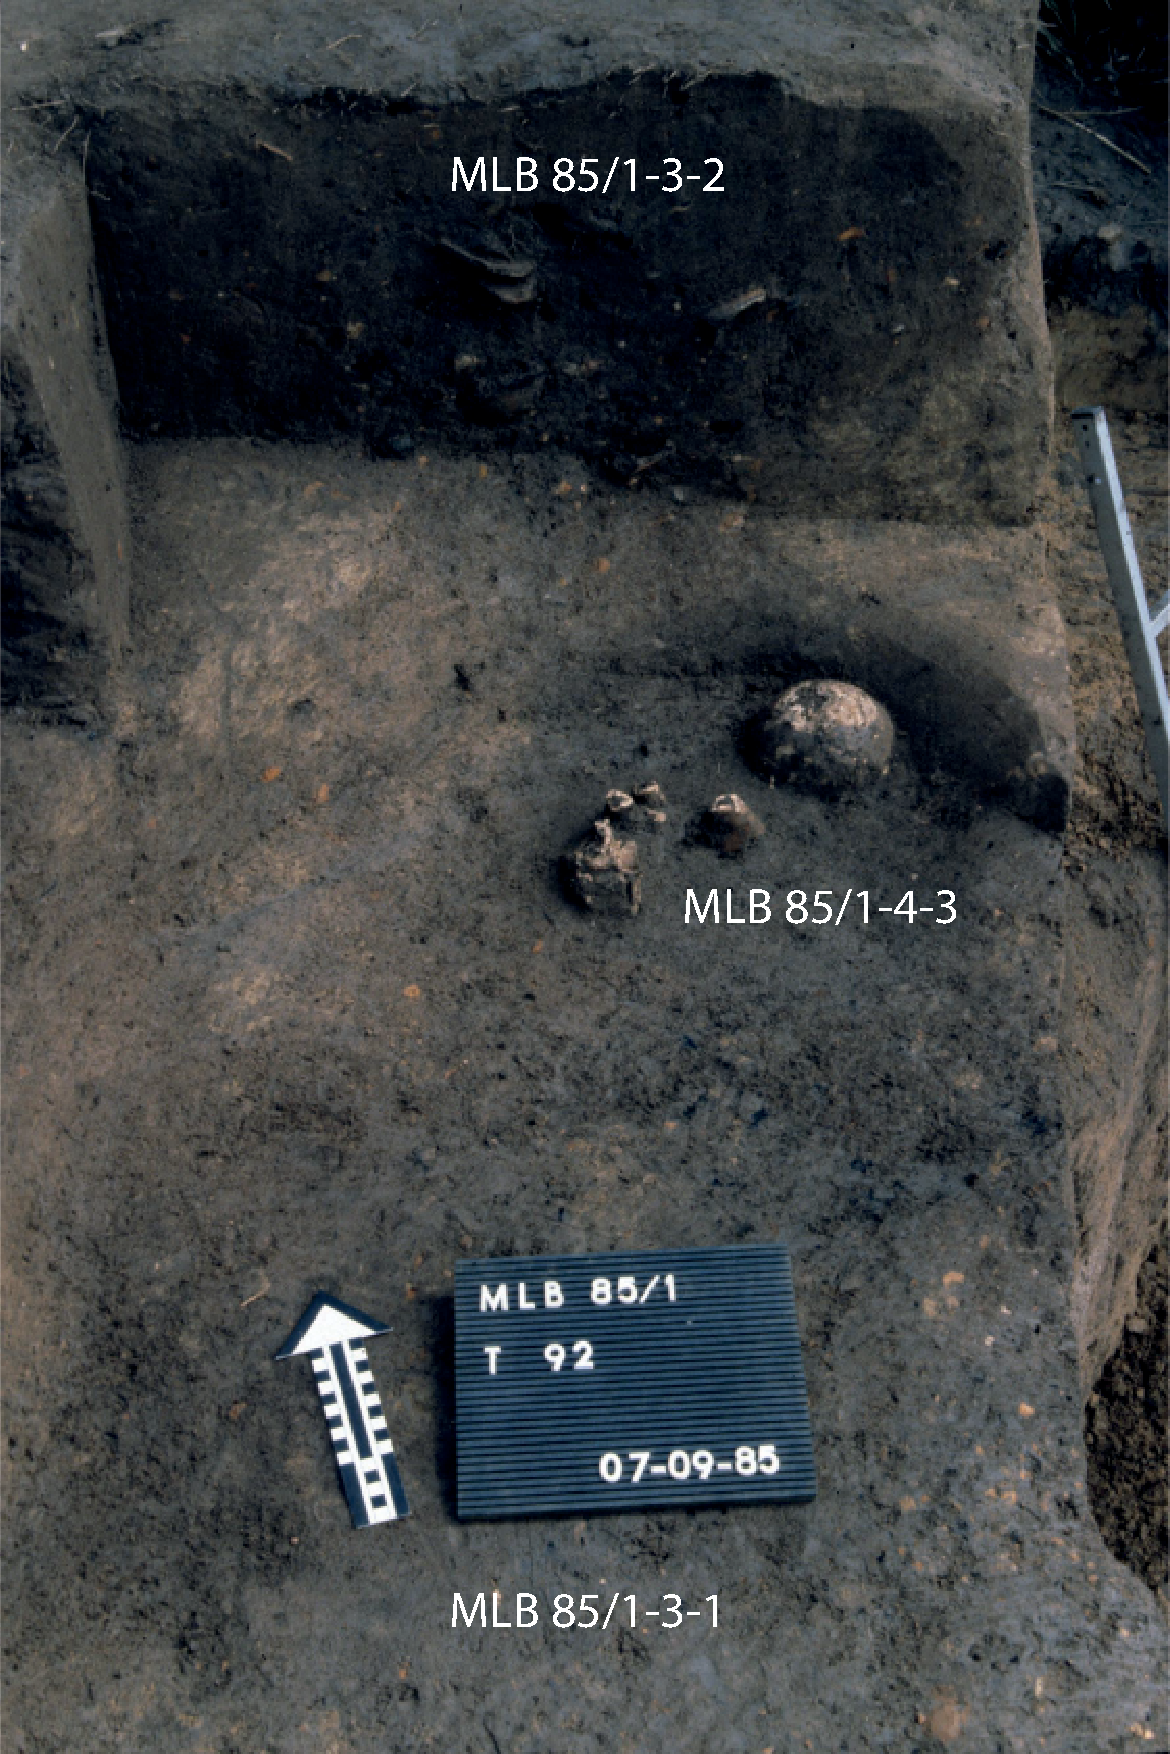
\includegraphics[width=\columnwidth]{fig/MLB85-1_Pl4_E85-031-34.pdf}
 \caption{Planum 4}
 \label{fig:MLB85-1_Pl4}
 \end{subfigure}\hfill
 \begin{subfigure}{\columnwidth}
 \centering
 \includegraphics[width=\columnwidth]{fig/MLB85-143_E85-032-10.jpg}
 \caption{Detail}
 \label{fig:MLB85-143_Detail}
 \end{subfigure}
 \caption{MLB 85/1-4-3: a) Planum 4 von Schnitt MLB 85/1 (T 92, Blick von Süden); b) Detail des Schädels (Blick von Osten; Fotos: M. K. H. Eggert, 1985).}
 \label{fig:MLB85-1_SekBest_Fotos}
\end{figure*}

\begin{figure*}[p]
\centering
\begin{subfigure}[b]{\textwidth}
\adjustbox{trim = 0 0 0 {.05\height}, clip}{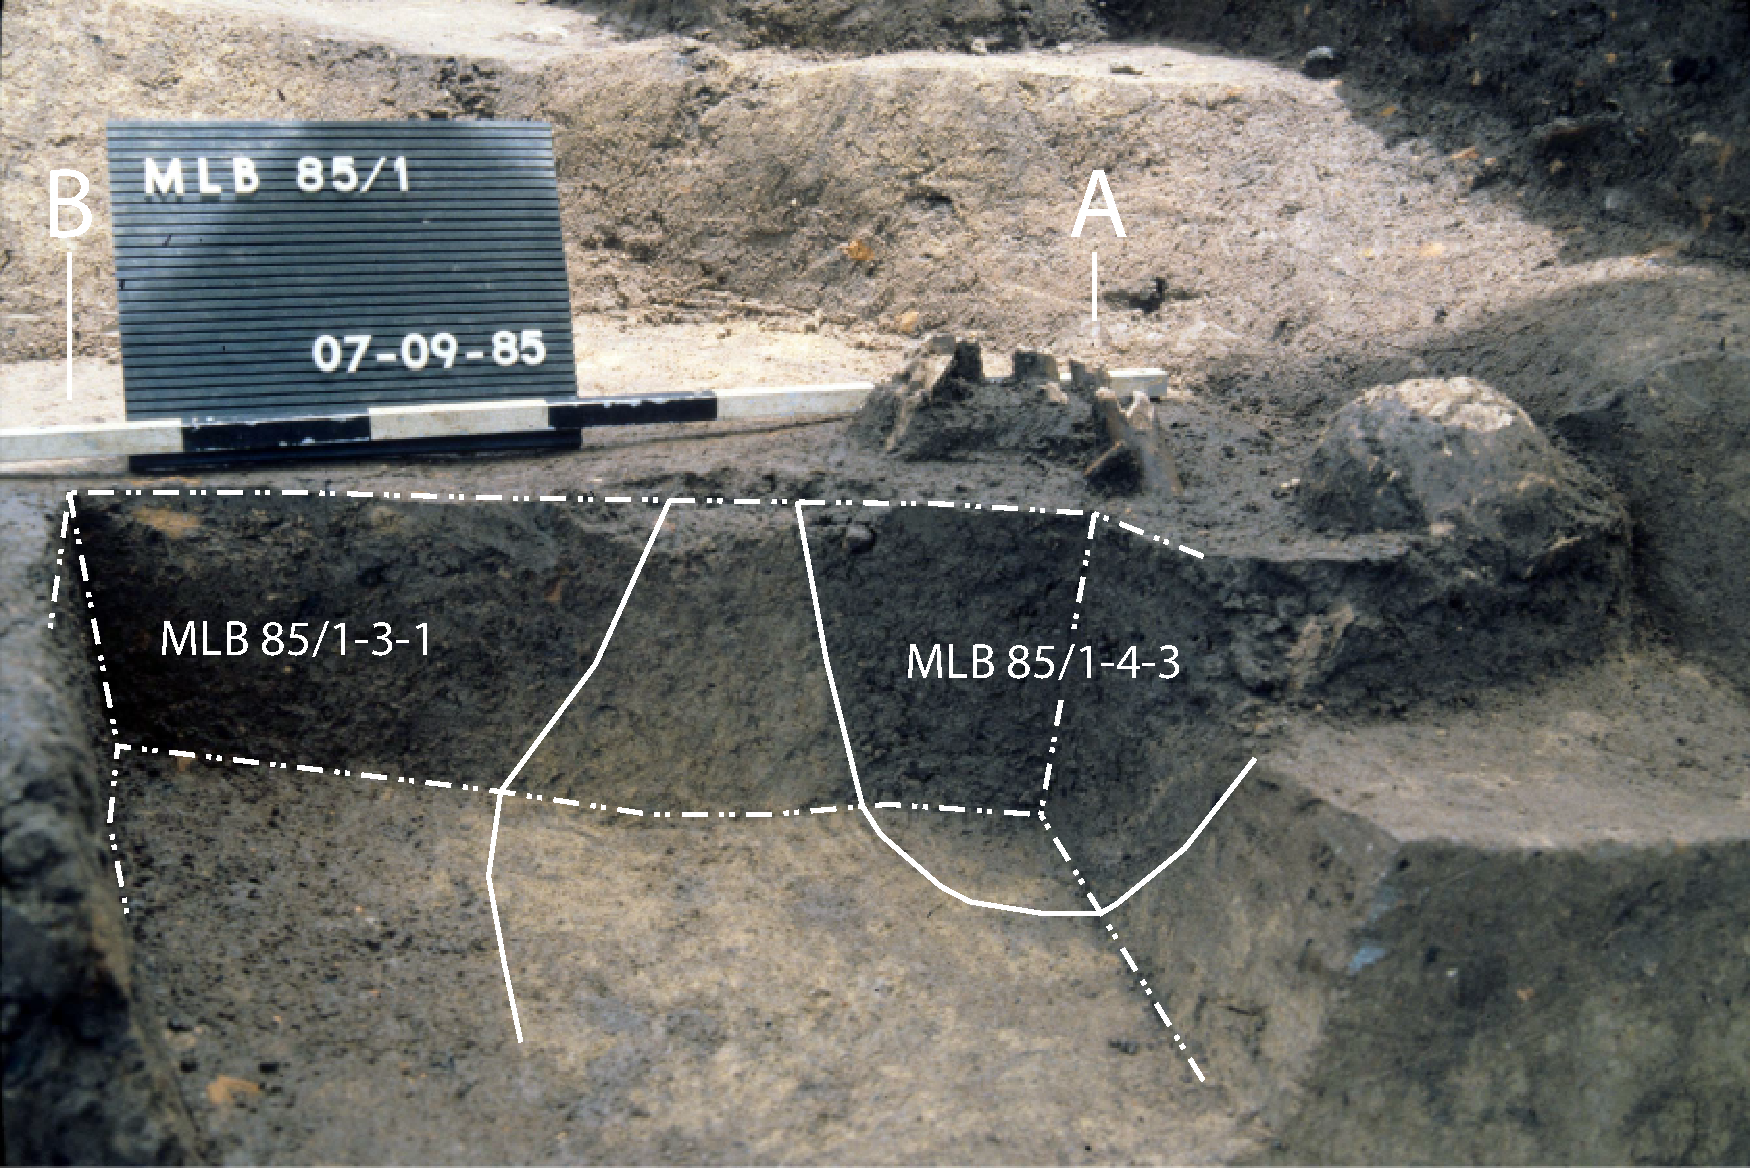
\includegraphics[width = \textwidth]{fig/MLB85-143_E85-032-05.pdf}}
\caption{Profil A--B, Blick von Südosten}
 \label{fig:MLB85-143_Prof_A-B}
 \vspace{1ex}
\end{subfigure}
\begin{subfigure}[b]{\columnwidth}
\includegraphics[width = \columnwidth]{fig/MLB85-143_E85-032-19.pdf}
\caption{Blick von Süden aus Profil E--F}
 \label{fig:MLB85-143_Prof_E-F_1}
\end{subfigure}\hfill
\begin{subfigure}[b]{\columnwidth}
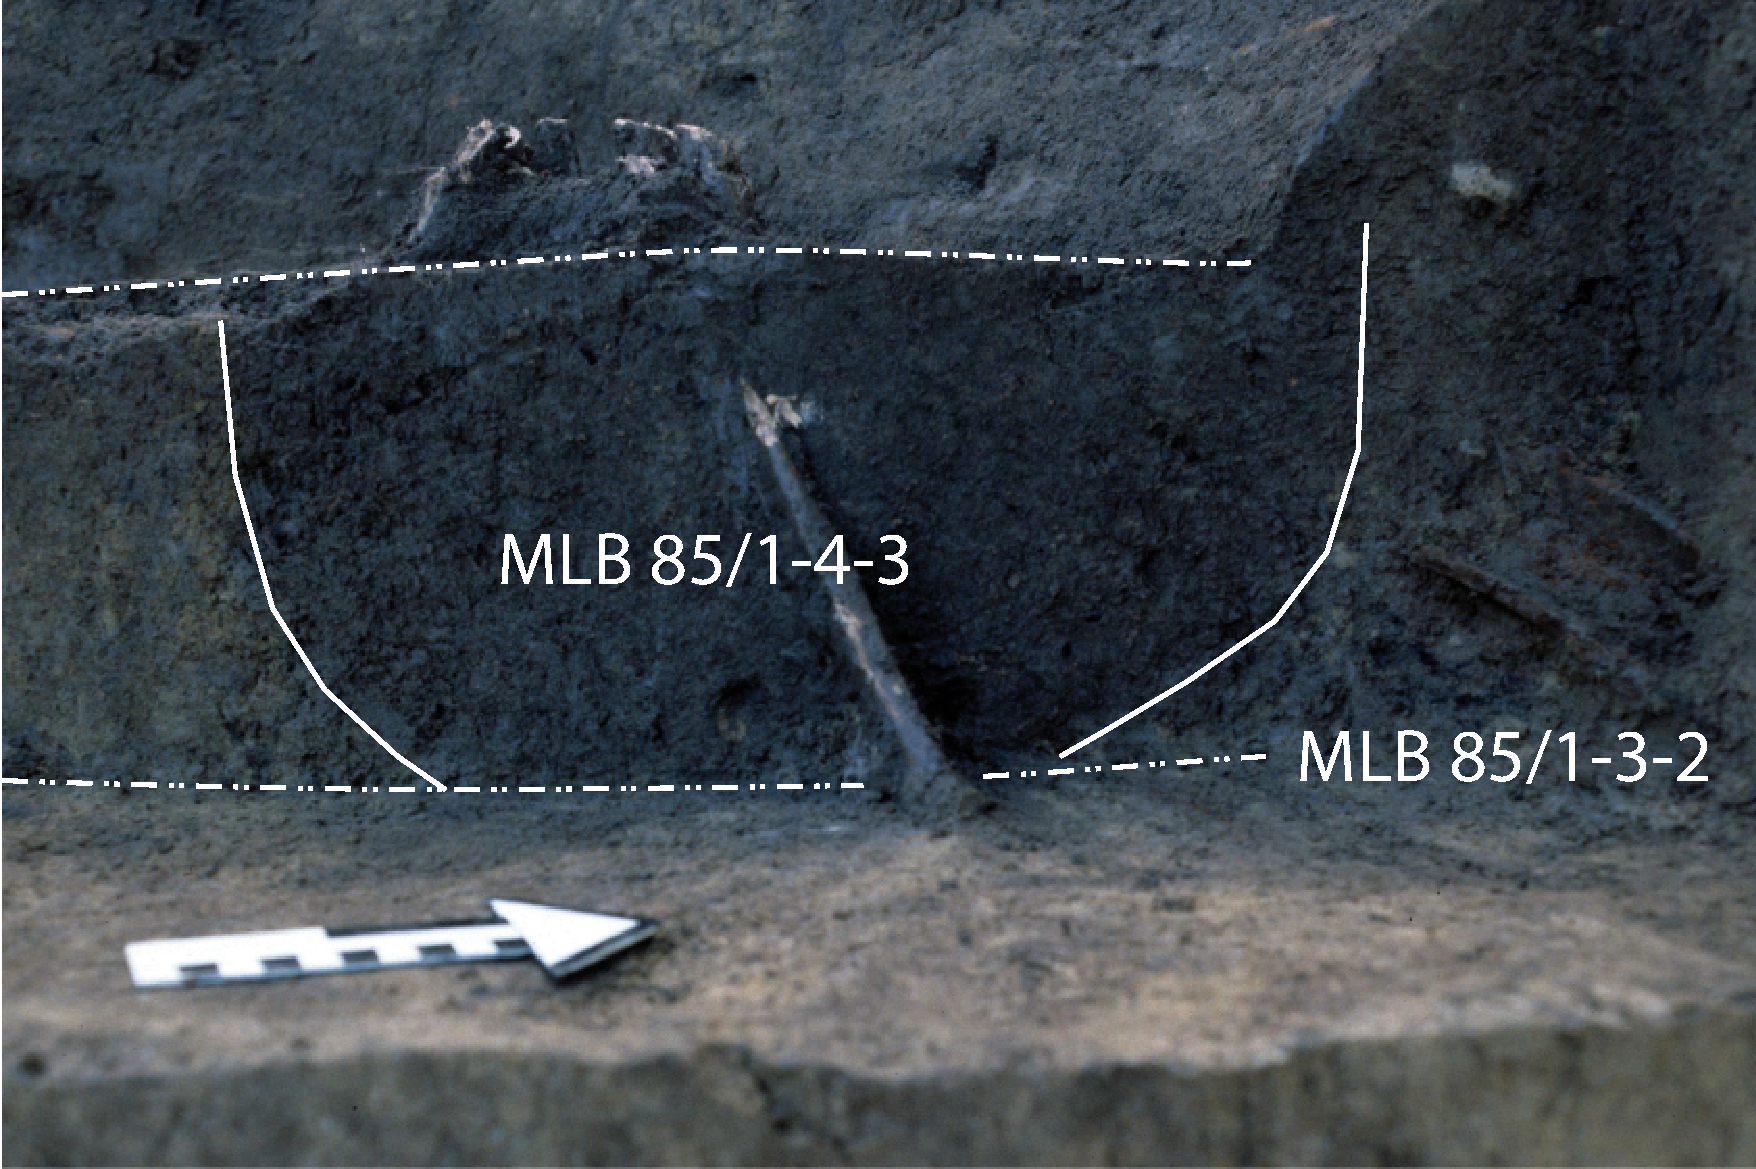
\includegraphics[width = \columnwidth]{fig/MLB85-143_E85-032-16.pdf}
\caption{Profil E--F, Blick von Ostsüdosten}
 \label{fig:MLB85-143_Prof_E-F_2}
\vspace{4.25ex}
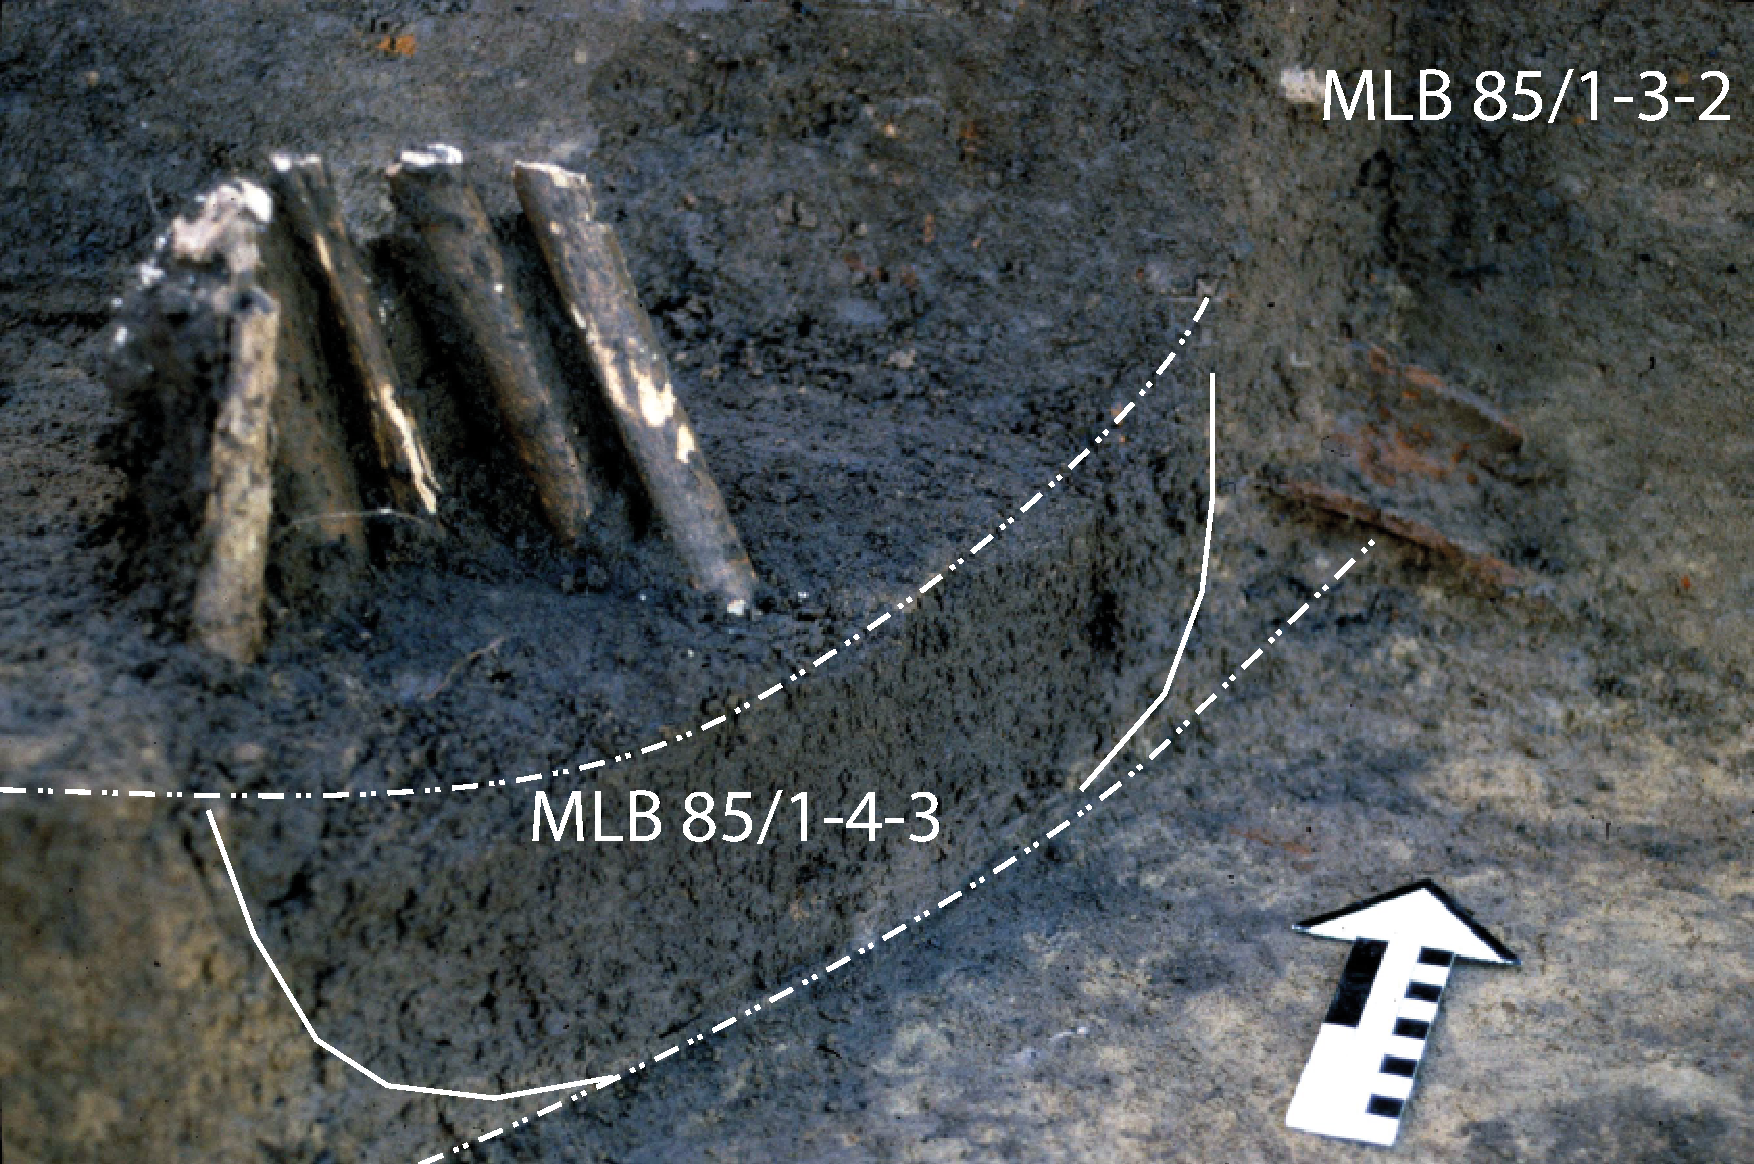
\includegraphics[width = \columnwidth]{fig/MLB85-143_E85-032-22.pdf}
\caption{Zurückverlegtes Profil E--F, Blick von SSO}
 \label{fig:MLB85-143_Prof_E-F_3}
\end{subfigure}
 \caption{MLB 85/1-4-3: Zurückverlegtes Profil E–F (siehe Abb.~\ref{fig:MLB85_1_Zeichnung}), welches die stratigrafische Überlagerung der nördlichen Grube MLB 85/1-3-2 durch die Sekundärbestattung zeigt  (Fotos: M. K. H. Eggert, 1985).}
 \label{fig:MLB85-143}
\end{figure*}

\section*{\begin{tabular*}{\linewidth}{@{}l @{\extracolsep{\fill}} r@{}}
		Nr.~3 & MLB~85/1-4-3\\
	\end{tabular*} 
}

\textsf{\textbf{Maluba (Lua; Fpl.~230)}}

\vspace{1em}

\noindent\begin{tabular}{@{}rl@{}}
	\textbf{Feldarbeit:} & \textbf{05.09.--07.09.1985 (F. Nikulka)} \\ 
	\textbf{Abb.:} & \textbf{\ref{fig:MLB85-1_SekBest_Fotos}--\ref{fig:MLB85-1_SekBest_Skelettbild}} \\
	\textbf{Tab.:} & \textbf{\ref{tab:MLB85_1-4-3_Zaehne}--\ref{tab:MLB85_1-4-3_14C}}\\
	\textbf{Taf.:} & \textbf{27.9} \\ 
	\textbf{Lit.:} & \textbf{\textsc{Eggert}~1987b} \\ 
\end{tabular}

\paragraph{Grabung und Befunde}\hspace{-.5em}|\hspace{.5em}%
In einer nur etwa 0,3\,$\times$\,0,3\,m großen Grube mit schräger Wandung, gerundeten Ecken und konvexer Basis im nördlichen Bereich des Befunds MLB~85/1-3-1 (Kat.-Nr.~1) fanden sich menschliche Skelettreste. Der Befund zeichnete sich bereits im dritten Abtrag ab und wurde im vierten Abtrag deutlich sichtbar (Abb.~\ref{fig:MLB85_1_PlanaT70+90_Foto}). Im auf dem großen Hinterhauptsloch (\textit{Foramen magnum}) liegenden Schädel steckten zwei lange Röhrenknochen, die nicht mehr genauer identifiziert werden können. \textit{Maxilla} und \textit{Mandibula} waren ebenfalls in den Schädel gedrückt. Etwa 15\,cm südwestlich des Schädels waren fünf große Röhrenknochen senkrecht in einem Halbrund dicht nebeneinander an der Wandung der kleinen Grube platziert (Abb.~\ref{fig:MLB85-1_SekBest_Fotos}).

Die Eingrabung ließ sich durch ein Querprofil deutlich erfassen (Abb.~\ref{fig:MLB85-143_Prof_A-B}; siehe auch Abb.~\ref{fig:MLB85_1_Zeichnung}: A--B--C--D). Die stratigraphische Relation zwischen der Sekundärbestattung und der Grube MLB~85/1-3-1 konnte jedoch nicht geklärt werden. Es zeigte sich aber, dass der Befund in die nördlich angrenzende Grube MLB~85/1-3-2 einschneidet (Kat.-Nr.~2; Abb.~\ref{fig:MLB85-143_Prof_E-F_2}).

\begin{figure*}[p]
	\begin{minipage}[b]{.4\textwidth}
 		\caption{MLB 85/1-4-3: Erhaltene Skelettelemente (grün: vorhanden, hellgrün: fragmentiert vorhanden und durch Fotos belegt).}\label{fig:MLB85-1_SekBest_Skelettbild}
	\end{minipage}\hfill
	\begin{minipage}[b]{.55\textwidth}
 		\includegraphics[width=\textwidth]{fig/MLB85-143_Skelettbild_2013-11-09.jpg}
	\end{minipage}
\end{figure*}

\begin{table*}[p]
	\centering
		{\footnotesize
			\begin{sftabular}{@{}cccccccccccccccc@{}}
				\toprule 
				M3 & M2 & M1 & P2 & P1 & C & I2 & I1 & I1 & I2 & C & P1 & P2 & M1 & M2 & M3 \\ 
				18 & 17 & 16 & 15 & 14 & 13 & 12 & 11 & 21 & 22 & 23 & 24 & 25 & 26 & 27 & 28 \\ 
				\midrule 
				$\bullet$ & $\bullet$ & $\bullet$ & $\bullet$ & $\bullet$ & $\bullet$ & $\star$ & $\star$ & - & - & $\bullet$ & $\bullet$ & $\bullet$ & $\bullet$ & $\bullet$ & $\circ$ \\ 
				$\star$ & $\circ$ & $\circ$ & $\star$ & $\bullet$ & $\bullet$ & $\star$ & $\star$ & - & - & $\bullet$ & $\bullet$ & $\star$ & $\circ$ & $\circ$ & $\star$ \\ 
				\midrule
				48 & 47 & 46 & 45 & 44 & 43 & 42 & 41 & 31 & 32 & 33 & 34 & 35 & 36 & 37 & 38 \\ 
				\bottomrule
		\end{sftabular}}
	\caption{MLB 85/1-4-3: Zähne ($\bullet$ = vorhanden, $\star$ = Wurzel vorhanden, Krone fehlt, $\circ$ = Krone lose vorhanden) -- (Ansicht: rechts – links).}
	\label{tab:MLB85_1-4-3_Zaehne}
\end{table*}

\begin{table*}[p]
\centering
		{\footnotesize \begin{sftabular}{@{}cccccc@{}}
				\toprule 
				M3 & M2 & M1 & M1 & M2 & M3 \\ 
				18 & 17 & 16 & 26 & 27 & 28 \\ 
				\midrule 
				2 & 3+ -- 4 & 5 -- 5+ & 5 -- 5+ & 4 & 2 -- 2+ \\ 
				- & 2 & 3 -- 3+ & 3 -- 3+ & 2 & - \\ 
				\midrule 
				48 & 47 & 46 & 36 & 37 & 38 \\ 
				\bottomrule 
		\end{sftabular}}
	\caption{MLB 85/1-4-3: Abrasionsgrad der Molaren nach \textcite[72 Abb.~3.9]{Brothwell.1981}.}
	\label{tab:MLB85_1-4-3_ZaehneAbrasion}
\end{table*}

\paragraph{Anthropologie}\hspace{-.5em}|\hspace{.5em}%
Die Knochen wurden 1986 durch P. Caselitz (Hamburg) begutachtet (\textsc{Caselitz} 1986) und im Appendix des die Feldarbeiten von 1985 entlang des \mbox{Ubangi} beschreibenden Aufsatzes von \textcite[144]{Eggert.1987c} kurz beschrieben.\footnote{Im Jahr 2013 erfolgte eine erneute Begutachtung und Beschreibung des Materials durch den Autor. Für die Diskussion zu dieser Bestimmungen danke ich Michael Francken (Tübingen).}

Das Inventar umfasst viele Bruchstücke des Hirnschädels (\textit{Neurocranium}), der auf den 1985 gemachten Grabungsfotos noch teilweise erhalten war (Abb.~\ref{fig:MLB85-1_SekBest_Skelettbild}), 2013 aber nur noch in stark fragmentiertem Zustand vorlag. Es fanden sich kaum Teile größer als 5\,$\times$\,5\,cm. Alle Fragmente weisen regelhaft sehr verrundete Bruchkanten auf. Die Oberflächen der Knochenfragmente sind stark angelöst. An zwei Bruchstücken sind \textit{endocranial} noch Nahtbereiche sichtbar, jedoch lässt sich nicht bestimmen, um welchen Nahtbereich es sich handelt. Vom Gesichtsschädel (\textit{Viscoerocranium}) waren nur sehr wenige, noch stärker fragmentierte Teile erhalten.

Ober- (\textit{Maxilla}) und Unterkiefer (\textit{Mandibula}) sind deutlich besser erhalten und liegen fast vollständig vor. Vom \textit{Ramus mandibulae} ist auf der rechten Seite jedoch nur der Ansatz vorhanden, links fehlt er völlig. Der Unterkiefer ist generell sehr robust. Im Oberkiefer liegt eine deutliche Prognathie im Bereich der Schneidezähne (\textit{Incisivi}) vor. Die beiden \textit{Incisivi} der linken Seite fehlen im Ober- wie im Unterkiefer komplett (Tab. \ref{tab:MLB85_1-4-3_Zaehne}). Von insgesamt acht Zähnen fehlen die Kronen und nur die Wurzeln sind erhalten. Bei einigen \textit{Molaren} liegen die Kronen separat vor, können aufgrund der Fragmentierung der zugehörigen Wurzeln aber nicht mehr angepasst werden. Die Zähne weisen eine deutliche Abrasion auf (Tab. \ref{tab:MLB85_1-4-3_ZaehneAbrasion}). Deutlich sichtbare Zahnengstellen zeigen sich zwischen dem zweiten \textit{Incisivus} (42) und dem \textit{Caninus} (43) im Unterkiefer auf der rechten Seite. Der zweite \textit{Incisivus} im Oberkiefer links (22) weist buccal einen möglichen Wurzelabszess mit Eröffnung des Knochens an der Wurzelspitze auf (\textsc{Caselitz} 1986). Der dritte \textit{Molar} im Oberkiefer links (28) ist in die Nasennebenhöhle durchgebrochen. Die \textit{Canini} und \textit{Prämolaren} im Unterkiefer zeigen Zahnsteinanlagerungen und fast alle Wurzeltaschen sind parodontitisch (\textsc{Caselitz} 1986). Die Abrasion der Kauflächen ist nicht besonders stark. Das Dentin ist nur an einigen Stellen sichtbar.

Von den Wirbeln ist lediglich der \textit{Arcus anterior} des Atlas mit der \textit{Fovea dentis} erhalten (\textsc{Caselitz} 1986). Das postcraniale Skelettmaterial besteht aus Diaphysenfragmenten der oberen und unteren Extremitäten. Epiphysenfragmente konnten nicht beobachtet werden. Es handelt sich um Reste beider \textit{Femora}, \textit{Tibie}, \textit{Fibulae}, \textit{Ulnae} sowie des rechten \textit{Radius} (Abb.~\ref{fig:MLB85-1_SekBest_Skelettbild}). Die Knochen machen allgemein einen eher grazilen Eindruck. Es lassen sich keine pathologischen Auffälligkeiten beobachten.\footnote{Maße, die beispielsweise für eine Körperhöhenrekonstruktion genutzt werden könnten, konnten aufgrund der Unvollständigkeit nicht abgenommen werden.} Zwischen den Knochen der rechten und linken Körperhälfte konnten keine Unterschiede beobachtet werden, somit kann davon ausgegangen werden, dass die \textit{endocranialen} Skelettteile von einem Individuum stammen. Die generelle Robustizität des Knochenmaterials legt den Schluss nahe, dass \textit{craniales} und \textit{endocraniales} Material zusammengehören und somit eine Auswahl der Skelettteile eines Individuums vorliegen.

\begin{table*}[!tb]
	\centering
	{\footnotesize \begin{sftabular}{@{}p{.125\textwidth}p{.15\textwidth}p{.4\textwidth}p{.2\textwidth}@{}}
			\toprule 
			\textbf{Lab-Nr} & \textbf{Datum (bp)} & \textbf{Datum (2-Sigma)} & \textbf{Probe }\\ 
			\midrule 
			Poz-62102 & 580 \( \pm \) 30 & \begin{tabular}[t]{@{}l@{}}1300--1369 n.~Chr. (63,6\,\%)\\ 1381--1419 n.~Chr. (31,8\,\%)\end{tabular} & Fibula \\ 
			Poz-62103 & 810 \( \pm \) 80 & 1030--1297 n.~Chr. & Ulna \\ 
			\bottomrule 
	\end{sftabular} }
	\caption{MLB 85/1-4-3: \textsuperscript{14}C-Datierungen.}
	\label{tab:MLB85_1-4-3_14C}
\end{table*}

Der Zahnbefund, mit den dritten \textit{Moralen} in der Kauebene und bereits leichter Abrasion, weist auf ein mindestens adultes Sterbealter des Individuums hin.\footnote{Angaben zu Alter und Geschlecht können ohne Kenntnis der Populationsvarianz nur grobe Schätzungen sein. Die hier gemachten Angaben sind nur als grobe Deutung beziehungsweise Ansprache der beobachteten Merkmale zu sehen.} Die Zahnkronenabrasion nach \textcite[72~Fig.~3.9]{Brothwell.1981} ergibt ein Sterbealter von 25--35, eventuell auch 35--45 Jahren.\footnote{Es muss an dieser Stelle auf das Fehlen von Vergleichen für zentralafrikanische Populationen hingewiesen werden. Da die Zahnkronenabrasion zentral von der konsumierten Nahrung abhängt, können die von \textcite{Brothwell.1981} gemachten Angaben nur einen groben Richtwert liefern.} Im Bereich des Nahtverschlusses des harten Gaumens ist lediglich der distale Bereich der AMP-Sutura und der Bereich der IN-Suturen erhalten, während der Bereich der TP-Naht zu fragmentarisch erhalten ist \parencites[siehe][]{Mann.1987}[782 Abb.~1]{Mann.1991}{Apostolidou.2011}. Dass die IMP-Naht nicht verstrichen, die IN-Naht hingegen verstrichen ist, deutet nach \textcite[783 Tab 1, Abb. 2]{Mann.1991} auf ein Sterbealter zwischen 20--25 und 50\textsuperscript{+} Jahren hin. Der \textit{endocraniale} Nahtverschluss, mit den teilweise noch sichtbaren Nähten unterstreicht diesen (spät)adulten bis maturen Befund. Ein Problem bereitet jedoch die Tatsache, dass sich keine Aussage bezüglich des Nahtbereiches, aus dem die Fragmente stammen, treffen lässt. Alles in allem deuten die beobachtbaren Merkmale auf ein tendenziell spätadultes Sterbealter, zwischen 25--45 Jahren hin.

Das nicht ausgeprägte Kinn kann als weibliches Merkmal interpretiert werden, ebenso wie der flache Winkel der \textit{Pars petrosa}.\footnote{Aufgrund der schlechten Erhaltung und fehlender Skelettelemente lässt sich die kombinierte Methode nach \textcite{Ferembach.1979} nicht anwenden. Eine Ansprache des Geschlechts des Individuums lässt sich nur auf Basis von Einzelmerkmalen vornehmen.} Die allgemeine Robustizität, die von Caselitz \parencite[siehe][144]{Eggert.1987c} als Hinweis auf ein männliches Geschlecht angeführt wird, ist bei Personen aus Afrika häufiger zu beobachten\footnote{Mündl. Mitt. M. Francken (2013).} und kann ohne Populationsdaten nur bedingt als Argument herangezogen werden.\footnote{Eine Geschlechtsdifferenzierung auf Basis der \textit{bukko-lingualen} Zahnkronendurchmesser nach \textcite{Alt.1998} wurde versucht. Sie erbrachte jedoch keine verwertbare Aussage, da die Populationsvariabilität unbekannt ist und Vergleichswerte für afrikanische Populationen fehlen. Die Zähne des Skeletts MLB~85/1-4-3 sind 5--40\% größer als die eines Individuums aus dem Befund LBT~98/9 in Lobethal am Sanaga in Südwestkamerun (\textsc{Francken} 2009).} Das Geschlecht des Individuums kann insgesamt nur als unbestimmt mit einer Tendenz zum Weiblichen angesprochen werden.\columnbreak

\paragraph{Keramik\vspace{.5em}}\mbox{}\\
\begin{tabular}{@{}lrl@{}}
	Bearbeitet:	& 76\,g & (100\,\%) \\ 
\end{tabular} 

\vspace{1em}
\noindent Unter dem Komplex MLB~85/1-4-3 sind insgesamt sieben Scherben mit einen Gesamtgewicht von lediglich 76\,g verzeichnet. Es handelt sich dabei größtenteils um Vertreter des Batalimo-Maluba-Stils. Jedoch fanden sich unter den nicht individuell beschrifteten, undiagnostischen Stücken auch Scherben des \textit{Fabrics} 7, welches für die am Fundplatz ebenfalls gefundene Keramik der Matoto-Gruppe charakteristisch ist (Kap.~\ref{sec:MAT-Gr}). In den Abträgen oberhalb des dritten Planums der Grube MLB~85/1-3-1 (Kat.-Nr.~1) wurden die Funde aus dem Bereich über der Sekundärbestattung MLB~85/1-4-3 nicht getrennt. Die in diesen Abträgen gefundene, nicht zur Batalimo-Maluba-Gruppe zugehörige Keramik könnte potenziell im Zuge der Anlage der Sekundärbestattung MLB~85/1-4-3 in Tiefen gelangt sein. Keramik, die potenziell den Stilgruppen Matoto und Bobulu (Kap.~\ref{sec:BBL-Gr}) zugerechnet werden kann, fand sich auch in den Abträgen 4--5 (Abb.~\ref{fig:MLB85-1_KeramikStilgruppen}).\footnote{Die Abträge 4--5 der Grabung MLB~85/1-3-1 wurden auf jener Tiefe angelegt, in der sich auch die Sekundärbestattung MLB~85/1-4-3 fand (Abb.~\ref{fig:MLB85_1_Zeichnung}).} Es kann als wahrscheinlich gelten, dass eben jene Scherben der Stilgruppen Matoto und Bobulu, die in den Abträgen 4 und 5 des Befundes MLB~85/1-3-1 gefunden wurden, im Zusammenhang mit der Anlage der Sekundärbestattung MLB~85/1-4-3 stehen. Die starke Fragmentierung und Mischung von Stilgruppen legt den Schluss nahe, dass das Material nicht als \textit{Beigabe} in den Befund gelangte, sondern lediglich ein Teil der Verfüllung ist.

\paragraph{Datierung}\hspace{-.5em}|\hspace{.5em}%
Zwei Proben von Knochenfragmenten\footnote{Von einem Fragment der Schädelkalotte konnte kein Kohlenstoff mehr extrahiert werden.} aus der Sekundärbestattung MLB~85/1-4-3 wurden im Jahr 2014 radiokohlenstoffdatiert. Eine Probe von der rechten Ulna und eine weitere der rechten Fibula ergaben eine Datierung in das 11.--15.~Jh. n.~Chr. (Abb.~\ref{fig:MLB85_1_14C-Kalibration}, Tab.~\ref{tab:MLB85_1-4-3_14C}).\footnote{Die unkalibrierten Datierungen zeigen innerhalb der zweifachen Standardabweichung keine Überschneidung. Auf Basis dieser Beobachtung könnte davon ausgegangen werden, dass die Knochen nicht im Zuge eines einzelnen Ereignisses deponiert wurden und eine Mehrphasigkeit des Befundes vorliegt. Vor dem Hintergrund der präsentierten archäologischen wie anthropologischen Auswertung ergeben sich jedoch keinerlei Hinweise auf ein solches Szenario. Das anthropologische Material zeigt keine Hinweise für die Repräsentanz mehrerer Individuen und wird die dreifache Standardabweichung zugrunde gelegt, zeigen die unkalibrierten Radiokohlenstoffalter eine Überschneidung von annähernd 100 Jahren.}  

\paragraph{Interpretation}\hspace{-.5em}|\hspace{.5em}%
Unter der Bezeichnung MLB~85/1-4-3 wurde eine -- in einer kleinen Eingrabung deponierte -- Sekundärbestattung eines geschlechtlich unbestimmten, tendenziell weiblichen Individuums, das im Alter von 25--45 Jahren verstorben ist, erfasst. Teile der großen Langknochen wurden aufrecht am Rand der kleinen Grube aufgestellt. Weitere Langknochen wurden in den Schädel gesteckt und dieser dann ebenfalls in der Grube deponiert.\footnote{Die primären Bestattungsriten lassen sich anhand des Befundes ebenso wenig rekonstruieren, wie die Zeit, die zwischen Primär- und Sekundärbestattung lag. Mögliche Vergleiche bieten die von \textcite[266--268]{Wotzka.1993} beschriebenen Bestattungssitten der Fali in Nordkamerun. Diese beinhalten eine Entnahme des Schädels des Verstorbenen aus der primären Grabgrube nach drei Jahren und erneute Bestattung in einem Gefäß an einem anderen Ort \parencite[268]{Wotzka.1993}.} Zwei an Knochenmaterial datierte Radiokohlenstoffproben stellen den Befund in das 11.--15.~Jh. n.~Chr. Die Datierungen aus der Bestattung stellen einen \textit{terminus post quem} für die Datierung der in der Verfüllung angetroffenen Matoto-Keramik dar (Kap.~\ref{sec:MAT-Gr}).